\subsection{Projektkosten}

Für die Berechnung der Projektkosten wird ein Stundensatz von 150.- CHF angenommen.

\begin{longtable}[]{@{}lrr@{}}
  \toprule
  \textbf{Phase}  & \makecell[r]{\textbf{Geplante} \\\textbf{Stunden}} & \textbf{Kosten}\tabularnewline
  \midrule
  \endhead
  Initialisierung &  64                       &  9'600.- CHF\tabularnewline
  Konzept         &  66                       &  9'900.- CHF\tabularnewline
  Realisierung    & 136                       & 20'400.- CHF\tabularnewline
  Abschluss       &  64                       &  5'400.- CHF\tabularnewline
  \midrule
  \textbf{Total:} & 286                       & 42'900.- CHF\tabularnewline
  \bottomrule
  \caption{Projektkosten}
\end{longtable}


\noindent
Die geplanten Projektkosten betragen somit \textbf{42'900.- CHF}.

\begin{longtable}[]{@{}lll@{}}
  \toprule
  \textbf{Kostenstelle} & \textbf{Jährliche Kosten}\tabularnewline
  \midrule
  \endhead
  Software              & Keine\tabularnewline
  .com Domain           & 20.- CHF\tabularnewline
  Hosting               & 1'800.- CHF\tabularnewline
  \midrule
  \textbf{Total:}       & 1'820.- CHF\tabularnewline
  \bottomrule
  \caption{Betriebskosten}
\end{longtable}


Für die Betriebskosten eines Hostings wird einen durchschnittlichen monatlichen
Preis von 150.- CHF angenommen, da das Deployment für dieses nicht vorgesehen
ist, ist dies eine von Damian Senn geschätzte Zahl.

\clearpage
\subsection{Break Even Analyse}\label{break-even-analyse}

\subsubsection{Gigboost}

Beim Modell «Gigboost» wird Benutzern eine Option angeboten bei der ihre
publizierten Gigs auf der Startseite sowie in Suchresultaten anderen Einträgen
bevorzugt dargestellt werden. Für einen Gegenpreis von 10.- CHF kann ein Benutzer
seinen Gig «boosten».

\begin{figure}[!htb]
  \centering
  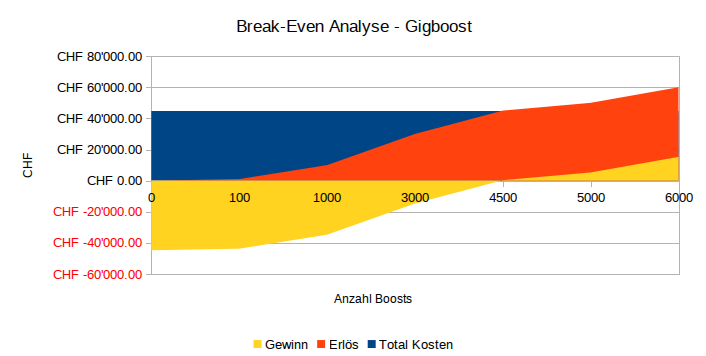
\includegraphics[width=0.95\textwidth]{initialisierung/wirtschaftlichkeit-gigboost.png}
  \caption{Break-Even Analyse - Gigboost}
\end{figure}

\clearpage
\subsubsection{Werbung}\label{break-even-analyse-werbung}

Im Modell «Werbung» wird ausgerechnet wieviele aktive Benutzer das Produkt benötigt
um in den nächsten Jahren Gewinn zu erzielen.

Durch Annahme von einem Erlös von \textbf{140.- CHF} pro \textbf{40'0000 Besucher}\footnote{\url{https://www.quora.com/How-much-does-Google-AdSense-pay-for-3-banners-on-a-webpage-per-1-000-views/answer/Manas-Sahu-59}} erhalten wir folgendes Bild:

\begin{figure}[!htb]
  \centering
  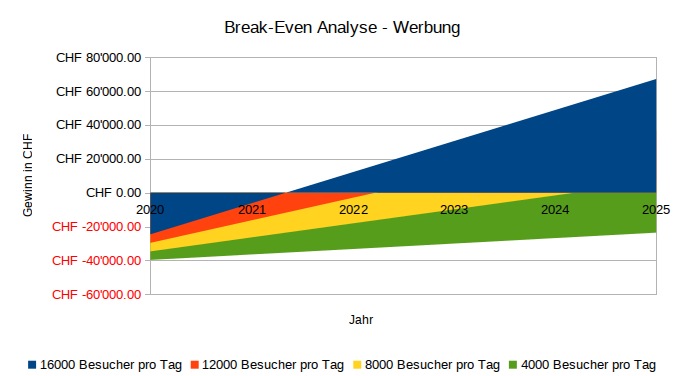
\includegraphics[width=0.95\textwidth]{initialisierung/wirtschaftlichkeit-werbung.png}
  \caption{Break-Even Analyse - Werbung}
\end{figure}

\begin{longtable}[]{@{}lll@{}}
  \toprule
  \textbf{Besucher pro Tag} & \textbf{Erlös pro Tag} & \textbf{Erlös pro Monat}\tabularnewline
  2'000                     & 7.- CHF                & 210.- CHF\tabularnewline
  4'000                     & 14.- CHF               & 420.- CHF\tabularnewline
  8'000                     & 28.- CHF               & 840.- CHF\tabularnewline
  12'000                    & 42.- CHF               & 1'260.- CHF\tabularnewline
  16'000                    & 46.- CHF               & 1'680.- CHF\tabularnewline
  \bottomrule
  \caption{Werbeeinnahmen pro Besucher}
\end{longtable}

Der Grafik ist zu entnehmen, dass das Produkt bei 8'000 Besucher pro Tag nach ca. 6 Jahren Gewinn erzielt. Bei 12'000 Besucher pro Tag erzielt das Produkt nach bereits 4 Jahren Gewinn und mit 16'000 Beucher pro Tag schon im dritten Jahr.
